% !TIKZEDT test = 3   
% !TIKZEDT BOUNDINGBOX = -3 -3  7  6 
 
 \usetikzlibrary{calc,through,intersections}

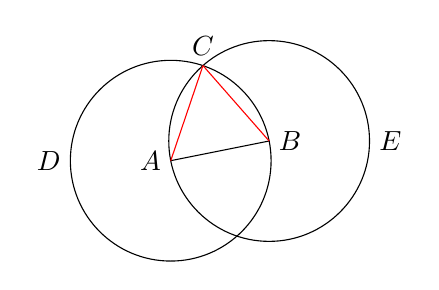
\begin{tikzpicture}

\coordinate [label=right:$B$] (B)at(1.25,0.25);
\coordinate [label=left:$A$] (A)at(0,0);

\draw (A) -- (B);

\node (D)[name path=D,draw,circle through=(B),label=left:$D$]at(A){};
\node (E)[name path=E,draw,circle through=(A),label=right:$E$]at(B){};


%Name the coordinates, but do not draw anything:
\path [name intersections={of=D and E}];
\coordinate [label=above:$C$](C)at(intersection-1);

%Now draw
\draw [red](A) -- (C);
\draw [red](B) -- (C);



\end{tikzpicture} 